\documentclass[11pt,letterpaper]{article}
\usepackage[margin=1.15in]{geometry}
\usepackage{times}
\usepackage[hyphens]{url}
\sloppy
\usepackage{graphicx}
\usepackage{booktabs}
\usepackage{amsmath}
\usepackage{amssymb}
\usepackage{natbib}
\usepackage[hidelinks]{hyperref}
\bibliographystyle{plainnat}
\frenchspacing
\setcounter{secnumdepth}{2}

\title{Three Ways an Elicited Evaluation Measures Its Own Design\\
\large Item sampling, instruction effects, and threshold artifacts,\\
with a worked case and 7{,}920 elicitations}

\author{
  Maikel Y. Leyva-V\'azquez\\
  {\small Universidad Bernardo O'Higgins, Santiago, Chile}\\
  {\small Universidad Bolivariana del Ecuador, Guayaquil, Ecuador}\\
  {\small Universidad de Guayaquil, Guayaquil, Ecuador}\\
  {\small \texttt{myleyvav@ube.edu.ec}}
}
\date{August 2026}

\begin{document}
\maketitle

\begin{abstract}
A large class of evaluations asks a language model to report a number about a
statement---a confidence, a rating, a degree---and treats that number as a measurement. We quantify three ways such a design measures itself rather than the model, on
$7{,}920$ elicitations across six frontier model families and two unrelated construct families.

First, item sampling. A rate computed on one statement is a property of that statement:
between-item standard deviations exceed the mean in four of five constructs, so a single-item probe carries a 95\% interval half-width of $\pm 0.41$ on
a $[0,1]$ rate. A published figure of $0.661$ from one sentence becomes
$0.222$ over ten; reaching $\pm 0.05$ takes $69$ items in one family and $20$ in the other.

Second, instruction effects, where the obvious ablation misleads. Deleting the sentence that
names the measured behaviour barely moves the result; deleting the surrounding framing removes it. Running only the first half would have exonerated the instrument.

Third, threshold artifacts. Models answer on a coarse grid, so a cut on a modal value
adjudicates by rounding: moving one cut from $0.60$ to $0.90$
changes a rate by a factor of $16$ without touching the data.

Replicating all three on an unrelated task shows that no magnitude transfers intact and that the
framing effect does not replicate in the mean, though it still moves the response shape, which
sharpens the rule. We state the design rule each implies and release both banks, the code and
every generation.
\end{abstract}

\section{The shape of the problem}

Consider an evaluation of the following kind. You have a construct---hallucination, refusal,
value conflict, ambiguity, harmfulness---and you want to know how often a model exhibits some
response to it. You write one or a few statements that instantiate the construct, you ask the
model a question about each, you record a number, and you report the rate. Variants of this
design are everywhere: verbalized confidence \citep{lin2022teaching}, self-reported
uncertainty, LLM-as-judge scoring \citep{zheng2023judging}, self-critique,
constitutional-style self-evaluation, and most bespoke probes built for a paper.

That the resulting numbers are treated as measurements without the apparatus measurement
usually requires is a concern raised both inside NLP \citep{bowmandahl2021} and from
measurement theory \citep{jacobs2021measurement}. The design has three failure modes that
are individually well known and jointly under-measured.
The items may not represent the construct. The instruction may produce the behaviour it
measures. And the decision rule may sit where the model's answers pile up. This paper measures
all three on one corpus, so that the three magnitudes can be compared against each other rather
than asserted in isolation, and then measures them again on a second corpus that shares the
design and nothing else, so that the three can be told apart from the subject matter.

The first corpus comes from a study of a four-valued logic, reported elsewhere
\citep{leyva2026ladder, leyva2026itembank}. That study's subject matter is not the subject
matter here; we use it because it happens to have the design features needed---a purpose-built
item bank with ten matched items per construct, six model families, an instruction that can be
ablated in two nested steps, and a decision rule that is a threshold on a sum. Readers who care
about the logic should read those papers. Readers who run elicited evaluations should find
everything they need here.

The second corpus was built for this paper and shares none of that content. It asks the most
ordinary elicited question there is---how confident are you that this statement is
true---over well-known and obscure facts, well-known and obscure falsehoods, and genuinely open
questions, with the same models, the same wordings and the same two nested ablations. It exists
because a methods paper resting on one subject matter cannot distinguish a property of the design
from a property of that subject matter, and Section~\ref{sec:replication} shows the distinction
is not academic: one of the three effects does not survive the move.

\paragraph{Relation to the companion papers.} This is a methods paper and it makes no claim
about the logic under test there. Its contributions are the three quantities below, the design
rules that follow from them, the ablation protocol in Section~\ref{sec:instr}, and the whole of
the second construct family, which is new data collected for this paper and appears in neither
companion. Where a number is reported in a companion paper we say so.

\paragraph{What is not new.} That elicitation format moves elicited confidence is established
\citep{protocolsens2026}, as is the unreliability of LLM judges \citep{coinflip2026}; that
prompt formatting alone moves accuracy by many points \citep{sclar2024quantifying}; that
few-item instruments are imprecise is elementary psychometrics \citep{cronbach1972}; and that evaluation results deserve intervals is argued directly for
language models by \citet{miller2024errorbars}. What we
add is the size of each effect measured on a common corpus, the fact that the second one
defeats the natural ablation, the conversion of the first into a number of items, and a
replication on an unrelated construct family that shows which of the three magnitudes
transfer---none of them---and why.

\section{Corpus}
\label{sec:corpus}

All results below come from elicitations against six frontier model families, one per vendor,
through a single router at temperature $1.0$: GPT-4o, Claude Sonnet 4, Llama 4 Maverick,
DeepSeek Chat, Qwen3 235B and Mistral Medium 3.1.

\begin{table}[t]
\centering \small
\begin{tabular}{llr}
\toprule
Study & Design & Elicitations \\
\midrule
\multicolumn{3}{@{}l}{\emph{Family I --- epistemic states, four components}} \\
Bank & 110 items $\times$ 6 models $\times$ 3 wordings & 1{,}980 \\
Triple & 110 items $\times$ 6 models $\times$ 3 reps & 1{,}980 \\
Pilot & 8 items $\times$ 6 models $\times$ 3 wordings $\times$ 10 reps & 1{,}440 \\
Ablation A & 60 items $\times$ 6 models, instruction reduced & 360 \\
Ablation B & 60 items $\times$ 6 models, framing removed & 360 \\
\addlinespace[2pt]
\multicolumn{3}{@{}l}{\emph{Family II --- factual confidence, one component}} \\
Factual bank & 60 items $\times$ 6 models $\times$ 3 wordings & 1{,}080 \\
Ablation A$'$ & 60 items $\times$ 6 models, instruction reduced & 360 \\
Ablation B$'$ & 60 items $\times$ 6 models, framing removed & 360 \\
\midrule
& & \textbf{7{,}920} \\
\bottomrule
\end{tabular}
\caption{The corpus. Family~I holds ten matched statements for each of five
constructs---ethical conflict, epistemic ignorance, vagueness, future contingency and logical
paradox---plus ten anchors of settled truth. Family~II (Section~\ref{sec:replication}) is an
unrelated task in the same elicited form: ten statements for each of five constructs---well-known
true, well-known false, obscure true, obscure false and genuinely open---plus ten arithmetic
anchors. Every generation is released.}
\label{tab:corpus}
\end{table}

In Family~I the outcome we track is a binary label derived from the reported numbers by a
threshold rule. Its content does not matter here; what matters is that it is a rate computed over
items, which is the form almost every elicited evaluation takes. In Family~II we report the
reported number itself, for a reason that is one of the findings: on that bank the threshold rule
destroys the measurement rather than summarising it (Section~\ref{sec:replication}).

\section{Item sampling: the rate is a property of the items}
\label{sec:items}

\begin{figure}[t]
\centering
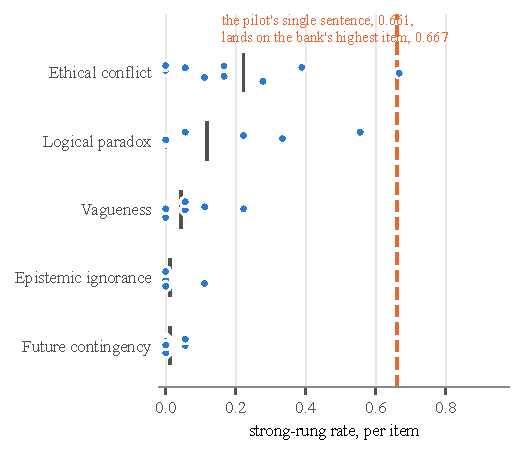
\includegraphics[width=0.72\linewidth]{fig1_between_items}
\caption{Rate for each of the ten items in each construct; the short bar is the construct mean.
Where the effect is large the spread is large. The dashed line is a published figure obtained
from a single statement, which lands on the highest of the ten items measuring the same
construct.}
\label{fig:items}
\end{figure}

That items differ in how much they tell you is the premise of the item-response work applied
to NLP leaderboards and test sets \citep{rodriguez2021evaluation, vania2021comparing};
what we add is the consequence for a rate reported over a handful of them.
Figure~\ref{fig:items} shows the rate for every item separately. The pattern is the finding:
\emph{the spread between items of the same construct is as large as the effect}.

\begin{table}[t]
\centering \small
\begin{tabular}{lccc}
\toprule
Construct & mean & SD between items & SD / mean \\
\midrule
Ethical conflict & 0.222 & 0.211 & 0.95 \\
Logical paradox & 0.117 & 0.193 & 1.66 \\
Vagueness & 0.044 & 0.073 & 1.65 \\
Future contingency & 0.011 & 0.023 & 2.11 \\
Epistemic ignorance & 0.011 & 0.035 & 3.16 \\
\bottomrule
\end{tabular}
\caption{Ten items per construct. The standard deviation between item means equals or exceeds
the construct mean in four of the five cases, and is of the same order in the fifth.}
\label{tab:sd}
\end{table}

The consequence is quantitative. A rate estimated from $k$ items has a standard error of
approximately $s/\sqrt{k}$, where $s$ is the between-item standard deviation of
Table~\ref{tab:sd}. Taking the largest construct, $s = 0.211$:

\begin{figure}[t]
\centering
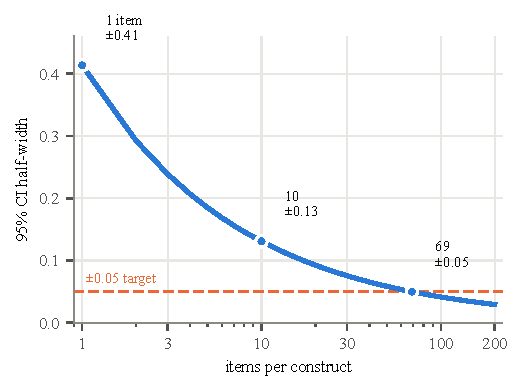
\includegraphics[width=0.72\linewidth]{figA_precision}
\caption{Precision of a construct-level rate as a function of items, at the between-item
standard deviation we measure. One item gives a 95\% interval half-width of $\pm 0.41$ on a
scale that runs from $0$ to $1$.}
\label{fig:precision}
\end{figure}

At one item the 95\% interval half-width is $\pm 0.41$. The interval is wider than most effects
anyone reports, which is another way of saying that a single-item probe of a construct like
this one is, to a first approximation, uninformative about the construct. Ten items give
$\pm 0.13$. Reaching $\pm 0.05$ takes $69$.

\paragraph{The worked case.} The corpus we borrow was preceded by a study using one statement
per construct, which reported a rate of $0.661$ for the construct we call ethical conflict
\citep{leyva2026ladder}. Measured over ten items the same quantity is $0.222$, and the per-item
values run from $0.000$ to $0.667$. The published figure is not a mismeasurement of its
sentence; it is an accurate measurement of the most extreme of ten, reported as though it
described the construct. This is the failure mode in its purest form, and we suspect it is
common precisely because nothing in the single-item result looks wrong.

\paragraph{Design rule.} Report the between-item standard deviation, not only the mean. If it
is of the order of the mean---and in five of five constructs here it was---then a difference
between two constructs is not interpretable without an interval that resamples \emph{items},
not evaluations. In our corpus the aggregate contrast survives such a bootstrap
($\Delta = 0.178$, $[0.058, 0.312]$) while the contrast against the nearest single construct
does not ($\Delta = 0.107$, $[-0.060, 0.272]$), and only the item-clustered interval reveals
the difference between those two situations.

\section{Instruction effects: ablate the framing, not the sentence}
\label{sec:instr}

Elicited evaluations carry an instruction that explains what is being asked. The instruction is
part of the measurement, and when the behaviour of interest is one the instruction mentions,
the natural worry is that the instruction produces it.

In our corpus the worry is concrete. The system message reads, in part: \emph{``These dimensions
are NOT constrained to sum to 1.0. A statement can be simultaneously partially true, partially
false, partially indeterminate and partially neutral.''} The study then measures how often
models report values whose sum exceeds one. The instruction names the outcome.

The natural response is to delete the offending sentences and re-run. We did that, and we also
ran a second condition that removes the entire framing---the expert role, the explanation of
what each dimension means---leaving a generic instruction to answer in JSON. Same $60$ items,
same six models, same user message, $360$ elicitations each.

\begin{table}[t]
\centering \small
\begin{tabular}{lccc}
\toprule
& full & permission & framing \\
& instruction & deleted & removed \\
\midrule
Target rate, contested items & 0.077 & 0.060 & \textbf{0.004} \\
\quad 95\% CI & [.052,.113] & [.038,.093] & [.001,.020] \\
Target rate, largest construct & 0.200 & 0.155 & \textbf{0.000} \\
Sum exceeds one & 0.973 & 0.947 & 0.696 \\
Sum equals exactly one & 0.027 & 0.049 & \textbf{0.304} \\
Rate on anchors & 0.000 & 0.000 & 0.000 \\
Unparseable responses & 0.6\% & 6.4\% & 7.5\% \\
\bottomrule
\end{tabular}
\caption{Two nested ablations of the instruction. Deleting the sentences that name the outcome
changes little. Removing the framing changes everything---and also withdraws the question.}
\label{tab:ablation}
\end{table}

Deleting the permission does almost nothing. The rate moves from $0.077$ to $0.060$ with
intervals that overlap across most of their length; on the largest construct, from $0.200$ to
$0.155$. Models exceed the bound at nearly the same rate when nothing has told them they may.
Had we stopped there, we would have concluded that the instruction was innocent.

Removing the framing takes the rate to $0.004$ and raises exact normalization from $2.7\%$ to
$30.4\%$. But this condition does not withdraw a permission; it withdraws the question. A model
asked for four unexplained numbers treats them as a distribution, because nothing has told it
they are anything else. The honest conclusion is neither that the instruction manufactures the
result nor that the result is independent of how it is asked: the behaviour is a property of
the framed question, and does not survive being asked in another language.

\paragraph{Why one ablation is not enough.} The two conditions disagree, and either alone would
have misled us. The minimal ablation says the instruction is innocent; the maximal one says it
is everything. Only the pair locates the effect---in the framing, not the licence---and only
the pair makes clear that the maximal condition is not a control but a different experiment.

\paragraph{Design rule.} Run two nested ablations, not one. Remove the smallest span of text
that names the outcome; separately, remove the framing that makes the question intelligible.
Report both. If they disagree, the effect lives between them, and the paper's claim must be
scoped to the framed question rather than to the model. Report parse failures per condition
too: ours rose more than tenfold, all of it from one model, which is a fact about that model
and not about the manipulation, but a reader cannot know that unless it is broken out.

\section{Threshold artifacts: the rule sits where the answers pile up}
\label{sec:thresh}

\begin{figure}[t]
\centering
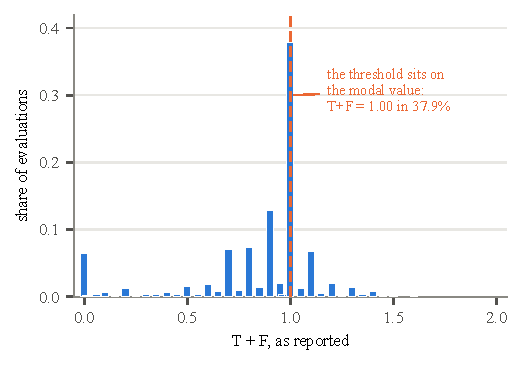
\includegraphics[width=0.72\linewidth]{figB_grid}
\caption{The quantity our decision rule thresholds, as reported. Models answer on a coarse
grid, and the threshold falls on the modal value.}
\label{fig:grid}
\end{figure}

Language models do not report continuous numbers. Across $7{,}852$ elicited components in this
corpus there are $46$ distinct values; $97.7\%$ are multiples of $0.05$ and $89.5\%$ are
multiples of $0.1$. The five most common values of one component account for $64\%$ of its
mass. This is a property of how models write numbers, not of the quantity being reported, and
it is stable across all four conditions we ran.

A decision rule that compares such a quantity against a fixed constant therefore adjudicates a
large share of cases by rounding. In our corpus the rule is a strict inequality against $1$,
and the quantity equals exactly $1.00$ in $37.9\%$ of evaluations---the modal value.
Figure~\ref{fig:grid} shows the pile-up sitting on the boundary.

That cutting a continuous quantity into two classes discards information and can mislead is a
long-standing result in psychological methods \citep{maccallum2002}; what is specific here
is that the cut point coincides with the value models return most often.
The consequence is not subtle. Replacing the strict comparison with a non-strict one---a change
no larger than the resolution at which models answer---moves the rate on the anchor condition,
which is the study's control, from $0.000$ to $0.778$. A result that had read as ``the signature
never fires on settled material'' turns out to be a statement about an inequality sign. The
ordering across constructs survives the perturbation, attenuated; the dramatic form of it does
not.

\paragraph{Design rule.} Before fixing a threshold, plot the distribution of the quantity it
cuts. If the cut point coincides with a modal value, report the rate under at least two
tie-breaking conventions and treat any conclusion that changes between them as a property of
the convention. Where the choice is free, place the threshold off-grid---at $1.025$ rather than
$1$---or use a margin, or report the underlying quantity instead of the label.

\section{A fourth, briefly: agreement across model families}
\label{sec:agree}

One further quantity is worth separating because it is routinely misread \citep{cohen1960, shroutfleiss1979}. Studies that use
several models as raters report an agreement coefficient over their labels. With one generation
per cell at a non-zero temperature, such a coefficient cannot distinguish models disagreeing
from a single model answering differently on a rerun.

Our corpus contains a design that separates them, because the pilot has ten repetitions. Over
the five contested statements, two repetitions of the same item by the same model under the same
wording land on different labels $17.5\%$ of the time ($n = 4{,}032$ pairs, 95\% CI
$[9.3,\,25.1]$); two different models answering the same item, wording and repetition disagree
$32.8\%$ of the time ($n = 2{,}240$ pairs, 95\% CI $[13.3,\,52.5]$). Roughly half of the
disagreement attributed to raters is stochastic variation a single rater produces on its own,
and that ratio is the stable part: it is $0.53$ over the contested statements and $0.52$ with
the three tautological controls added back, although adding them halves both rates. The
intervals are wide because the pilot has five contested statements, which is the first result
of this paper applied to itself; the decomposition is reproduced by
\texttt{family1/analyze\_pilot\_agreement.py}. The pooled coefficient over the bank, $\kappa = 0.184$ \citep{fleiss1971}, should be read
as a bound on reproducibility rather than as a measure of inter-model disagreement.

\paragraph{Design rule.} Either include repetitions and decompose, or report the coefficient as
a reproducibility bound and say why. Do not describe distinct model families as interchangeable
raters; they are different instruments, and the coefficient is not inter-rater reliability in
the sense the term usually carries.

\section{Replication on a second construct family}
\label{sec:replication}

The three results above come from one corpus about one subject matter. If they are properties of
the elicited design rather than of that subject matter, they should reappear in a task that
shares the design and nothing else.

So we built a second bank. The construct is factual confidence: the model is shown a statement
and reports a single number in $[0,1]$ for how confident it is that the statement is true. This
is the most ordinary elicited evaluation there is, and the quantity that the calibration
literature reports constantly. Five constructs of ten matched items each---well-known true,
well-known false, obscure true, obscure false, and genuinely open questions with no known
answer---plus ten arithmetic anchors. Same six model families, same three wordings, same two
nested instruction ablations. Nothing about four-valued logic appears anywhere in it.

The bank behaves. Parse failure is $0.0\%$ over $1{,}080$ elicitations, the arithmetic anchors
return exactly $1.000$ and $0.000$, and where ground truth exists the models are well calibrated
(Brier $0.005$). Whatever the bank measures, it is not noise.

\paragraph{The outcome we chose first was the artifact.} We initially tracked a
\emph{high-confidence rate}: the fraction of elicitations at or above $0.9$. That is the
domestic analogue of an overconfidence rate and the form in which such results are almost always
published. On this bank it is close to useless. Four of the five constructs pin to $0.000$ or
$1.000$ with zero between-item variance, and the one construct with real dispersion---the open
questions, where models spread from $0.42$ to $0.74$ across items and disagree with each other by
$0.120$---collapses to a rate of $0.028$. The signal is not absent. The threshold removes it.

That is Section~\ref{sec:thresh} arriving unbidden in a new domain, and it is worth stating in the
form a practitioner will meet it: \emph{the binarisation is not a summary of the measurement, it
is a second measurement, and on this bank it is the one that fails}. We therefore report the
continuous quantity as primary throughout this section and keep the rate only to show what it
costs.

\begin{figure*}[t]
\centering
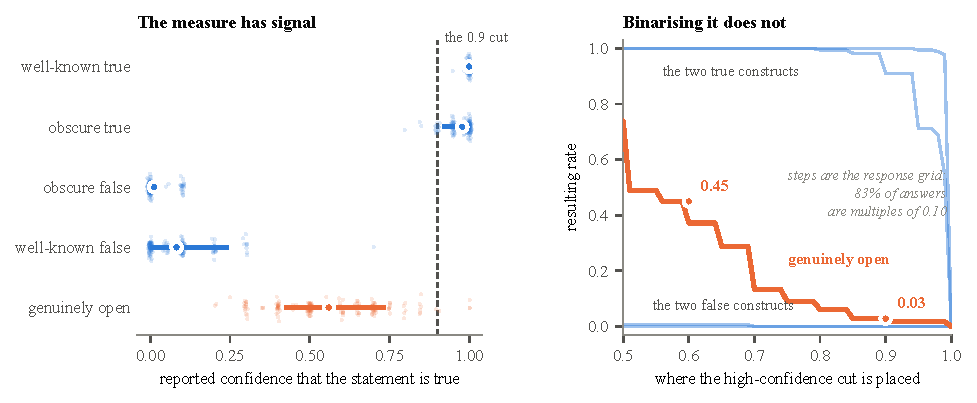
\includegraphics[width=\linewidth]{figC_threshold}
\caption{Second bank, $1{,}080$ elicitations. Left: reported confidence per elicitation, with the
item means spanned by the bar. The open-question construct occupies the middle of the scale and
spreads across items. Right: the rate that survives binarisation, as a function of where the cut
is placed. Moving the cut from $0.60$ to $0.90$ takes the open-question rate from $0.450$ to
$0.028$ without touching the data.}
\label{fig:threshold2}
\end{figure*}

\subsection{Item sampling replicates, and gives the rule its real shape}

Measured on the continuous scale, the between-item standard deviation within a construct ranges
from $0.001$ to $0.112$. Converted to a sample size for a $\pm 0.05$ half-width, that is between
$1$ and $20$ items \emph{within a single bank}---and the same calculation on the first corpus
returned $69$.

This is a stronger form of the rule than Section~\ref{sec:items} could state on its own. The
finding is not that between-item variance is large. It is that the number of items a construct
needs varies by a factor of nearly seventy across ordinary evaluation targets, with no way to
tell in advance which kind you have. Our own open-question construct needed $20$ items and we
gave it $10$; its interval is correspondingly wide, $[0.496,\,0.624]$.

\subsection{Instruction effects do not replicate in size, and the reason sharpens the rule}
\label{sec:instr2}

The second bank carries the same two nested ablations. Condition~A$'$ deletes the sentence that
licenses hedging---\emph{you are NOT required to commit to a verdict: when the evidence is
insufficient or the question is genuinely open, report a confidence near 0.5}. Condition~B$'$
deletes the surrounding role and scale as well, leaving only \emph{you are a careful evaluator}.
Both are paired: same items, same models, same wording, $360$ elicitations each, $100\%$ parse
rate in all three conditions.

The first half replicates exactly. Deleting the licence moves the open-question construct from
$0.551$ to $0.531$, a paired difference of $-0.020$ with a $95\%$ interval of
$[-0.057,\,+0.013]$. That is the first corpus's result again: the sentence that names the
measured behaviour is worth almost nothing.

The second half does not replicate at all. Deleting the entire framing moves the same construct
to $0.533$---a paired difference of $-0.018$, interval $[-0.052,\,+0.016]$. On the first corpus
the corresponding ablation took the headline quantity from $0.077$ to $0.004$. Here it does
nothing.

\paragraph{Why, and why it was predictable.} The two system messages are not equally load-bearing,
and the asymmetry is structural rather than empirical. In the first corpus the system message
carried the whole conceptual apparatus---four independent components not constrained to sum to
one---which the model cannot reconstruct from the question alone; removing it removed the task.
Here it carries a role label and a scale that the user turn already restates, since the question
is \emph{how confident are you that this statement is true} and already asks for \emph{a single
number in $[0.0, 1.0]$}. There was very little in it to delete.

We state this because it is the useful generalisation, and because stating it after seeing the
number would be worth less: \emph{framing is worth what the model could not have inferred without
it}. For an exotic elicited construct that is everything. For a familiar one it is close to
nothing. The design rule is unchanged---run both nested ablations---and is now better motivated,
because the two corpora are the two regimes and nothing short of running the ablation
distinguishes them in advance.

\paragraph{A second reason the mean was the wrong summary.} The instruction does change behaviour
on this bank. It does not change the mean. On the open-question construct the share of answers at
exactly $0.50$---the value the licence sentence explicitly names---falls from $17/60$ under the
full instruction to $9/60$ under \emph{both} ablations, a paired difference of $-0.133$ with
intervals $[-0.233,\,-0.050]$ for the full ablation and $[-0.267,\,+0.000]$ for the minimal one.
The standard deviation of the same answers rises from $0.161$ to between $0.195$ and $0.219$. The
instruction is read and obeyed; it redistributes mass symmetrically about the midpoint, so the
mean absorbs it and reports nothing.

With sixty elicitations per cell and one wording this is an indication rather than an established
effect, and one of the two intervals touches zero. We report it because the direction is identical
under both ablations and because the methodological point does not depend on the significance of
this particular pair: \emph{an ablation that reads null on the summary statistic can be large on
the distribution the statistic summarises}. Section~\ref{sec:instr} would have concluded that the
framing does not matter here. It matters; it moves the shape and not the location.

\paragraph{Design rule.} Run both nested ablations, and evaluate each against more than one
functional of the response distribution---at minimum a location statistic and one shape statistic
such as the mass on a focal value or the dispersion. Report the ablation as null only if it is
null on both.

\subsection{Threshold artifacts replicate, larger}

Models answer this bank on the same coarse grid: $26$ distinct values across $1{,}080$
elicitations, $95.7\%$ multiples of $0.05$ and $86.4\%$ multiples of $0.1$, with $33\%$ of answers
at exactly $1.00$ and $29\%$ at exactly $0.00$. Figure~\ref{fig:threshold2} shows what a cut does
to that.

\begin{table}[t]
\centering \small
\begin{tabular}{lcccc}
\toprule
& \multicolumn{2}{c}{continuous} & \multicolumn{2}{c}{rate at $\ge 0.9$} \\
\cmidrule(lr){2-3}\cmidrule(lr){4-5}
Construct & mean & SD b/w models & rate & SD b/w models \\
\midrule
well-known true  & 0.999 & 0.001 & 1.000 & 0.000 \\
obscure true     & 0.978 & 0.017 & 0.983 & 0.031 \\
obscure false    & 0.012 & 0.022 & 0.000 & 0.000 \\
well-known false & 0.083 & 0.049 & 0.000 & 0.000 \\
genuinely open   & 0.560 & 0.110 & 0.028 & 0.054 \\
\bottomrule
\end{tabular}
\caption{The same five constructs measured two ways. On the continuous scale the open-question
construct is the one with dispersion to explain; after binarisation at $0.9$ it is
indistinguishable from the two false constructs, all three reading as a rate near zero.}
\label{tab:twoways}
\end{table}

The size of the artifact is a factor of $16$: the open-question rate is $0.450$ at a cut of
$0.60$, $0.089$ at $0.80$, and $0.028$ at $0.90$. None of those numbers is more correct than the
others, and a paper reporting any one of them alone would be reporting its own threshold.

\subsection{Agreement replicates, and is construct-specific}

The second bank has no repetitions, so it cannot decompose rater variance the way
Section~\ref{sec:agree} does. What it has instead is three wordings, which isolates a different
component: how much a single model moves when the question is rephrased. That movement is $0.021$
in mean absolute confidence, against $0.048$ between different models on the same item---a ratio
of $0.44$, close to the $0.52$ the first corpus gives for repetition against models. Two designs,
two different intra terms, the same conclusion: a substantial share of what gets attributed to
model disagreement is not model disagreement.

The new observation is about pooling. Between-model dispersion on this bank runs from $0.001$ on
well-known truths to $0.120$ on open questions, a factor of $120$. An agreement coefficient
computed over a whole bank averages those together and reports a number that describes no
construct in it. Agreement is a property of the item, not of the panel.

\paragraph{Design rule.} Report agreement per construct, or not at all. If a single pooled
coefficient is reported, state the range it was pooled over.

\paragraph{What the second family shows.} Three of the four quantities reappear in a task with no
shared content, and the one that reappears largest is the one we had ranked third. The fourth,
instruction framing, does not reappear at all in the size the first corpus gave it---and that
non-replication is the most useful thing in this section, because it identifies what the effect
depends on. Framing is worth what the model could not have inferred without it, which is
everything for an exotic construct and nearly nothing for a familiar one.

What transfers, then, is the protocol and not a single magnitude. The item count moves from $69$
to $20$; the threshold effect grows from a factor of $2$ to a factor of $16$; the framing effect
falls from decisive to undetectable in the mean while remaining visible in the shape. Every one of
those numbers would have been wrong if borrowed from the other family. That is the argument for
measuring them rather than citing them, and it is the reason we ran a second bank instead of
asserting that the first one generalises.


\section{What this does and does not show}

Three magnitudes, two construct families, and no magnitude that transfers between them. Item
sampling sets a floor of roughly seventy items for a $\pm 0.05$ estimate in the first family and
twenty in the second. Threshold placement is worth the difference between $0.000$ and $0.778$ on
a control condition in the first, and a factor of sixteen in the second. Instruction framing is
worth everything in the first and nothing in the mean in the second, where it still moves the
shape of the response without moving its location; the reason---framing is worth what the model
could not have inferred without it---is the most portable thing in the paper. What generalises is the obligation to measure these three quantities, not any value they
took here.

The limits are worth stating plainly. Six models at one point in time, one generation per cell
in the main studies, and between-item standard deviations estimated from ten items each: these
are offered as an order of magnitude, not as constants. The within-cell variation that matters
for the first and third results is estimated from the pilot rather than measured in the bank.
The shape finding in Section~\ref{sec:instr2} rests on sixty elicitations per cell and is
reported as an indication. And nothing here licenses any claim about model internals: every
quantity is a property of text produced under an instruction.

\paragraph{The construct labels are ours, and the results do not rest on them.} We wrote the
items and we assigned them to constructs, so a reader is entitled to ask who says that these ten
statements measure ethical conflict rather than something else. That question is the classical
one of construct validity \citep{cronbachmeehl1955, messick1995}, and it arrives here in
the form measurement theory gives it for computational systems \citep{jacobs2021measurement}. The honest answer is that we do, and that the assignment has not
been validated against independent judges. What we can say is more limited than we first wrote, and the limit runs in a direction worth
setting out.

In the first family the second and third results are manipulations of the instrument---an
instruction deleted, a threshold moved---applied to a fixed set of items, and there the labels
are not load-bearing: the same statements are asked twice and the difference is the effect.

In the second family they are load-bearing, and we were wrong to imply otherwise. Both effects
live entirely on the open-question construct. On the four settled constructs the answers are
pinned near $0$ or $1$, where moving a threshold changes nothing and deleting an instruction
changes nothing, and Table~\ref{tab:twoways} shows exactly that. So the existence of those two
effects depends on that subset really consisting of questions with no settled answer. If those
ten items are not genuinely open, the effects do not shrink---they have nowhere to occur.
That is a construct-validity dependency at the centre of the replication, and the classification
instrument we release covers the first family's items and not these, which is the gap a reader
should hold against us first.

The first needs a qualification we would rather state than have extracted from us. A group
wrongly named still has the dispersion we report, so the measurement stands; but the rule drawn
from it---that reaching a $\pm 0.05$ half-width takes sixty-nine items---is an inference about
estimating a \emph{construct-level} quantity, and it presupposes that the items sample one. If
they do not, the between-item standard deviation mixes variability among items that do belong to
a construct with heterogeneity among items that do not, and we cannot say in which direction
that moves the estimate: a heterogeneous group is not guaranteed to be more variable than the
construct it was meant to sample. What follows is weaker and more useful than an upper bound.
The sixty-nine is a property of \emph{this bank}, not a constant of the construct, and it stays
that way until the assignment is validated. Which is the rule anyway: measure the dispersion in
your own bank rather than borrow ours. Construct labelling would matter for a claim of the form ``models behave
differently on ethical conflict than on vagueness'', and the one such contrast we report, in the
first family, we report as not established. To let others check the labelling rather than take
it on trust, the release includes two blind classification instruments, one per family: the items in
randomised order with the anchors mixed in unannounced, the category definitions, and the script
that returns agreement between raters and against our assignment. The second family gets a
narrower question than the first---whether a statement has a known answer or is genuinely
open---because that is the distinction its results rest on. Neither has been run.

What the results do support is narrow and, we think, useful: that these three failure modes are
not hypothetical, that their sizes are comparable to the effects such studies report, and that
the ablation protocol in Section~\ref{sec:instr} would have led us to the wrong conclusion if
we had run only its first half.

\section*{Declarations}

\paragraph{Ethics approval and human participants.} This study involved no human or animal
participants. Every observation in both construct families is a text generation produced by a
commercial language model through a programmatic interface, elicited by prompts written by the
author. No survey, interview, annotation task or crowdworker judgment was collected, and no
personal data were processed. Ethics committee approval and informed consent were therefore
not applicable.

\paragraph{Use of language models.} Language models are the object of study here rather than an
aid to writing: the corpus consists of their outputs, collected between 24 and 26 August 2026
through a single router at temperature $1.0$. Vendors and model families are named in
Section~\ref{sec:corpus}, and every released generation records the model family that produced
it. Exact provider version strings are recorded only for the pilot file; the router resolved
them at call time and the remaining files carry the family label rather than the resolved
version. Collection dates are given here and not per record. These results are properties of
specific model versions at a specific date and should not be assumed stable across releases, so
this is a limitation of the release rather than a detail: an exact re-run of the same versions
is not possible from what we published.

\paragraph{Competing interests.} The Family~I corpus was collected for two companion studies
co-authored by the present author, and one published figure re-analysed here ($0.661$) comes
from that work. This paper reports that the figure does not survive a larger item sample. No
other competing interests are declared.

\paragraph{Funding.} This research received no specific grant from any funding agency in the
public, commercial or not-for-profit sectors.

\section*{Data and code availability}

Both item banks, the elicitation and analysis scripts, and all $7{,}920$ raw generations
including response text are public at
\url{https://github.com/mleyvaz/elicited-evaluation-design}. Every figure and table here is
produced by released code from released data. Code is MIT-licensed; the banks and the
generations are CC BY 4.0.

The Family~I generations were collected for the companion studies rather than for this paper.
They are reproduced in full so that every number here can be checked in one place, with their
provenance stated in the repository; the citable source for that bank, together with an
independent re-analysis script written by a party that did not author the studies, remains
\url{https://github.com/mleyvaz/paraconsistent-signature-itembank}.

The second bank is released in the form in which it was analysed, including the first version of
its analysis script. That script took the high-confidence rate as its primary outcome, which
Section~\ref{sec:replication} reports as the artifact it turned out to be; we keep it in the
repository rather than quietly replacing it, because the sequence is part of the evidence for the
third design rule.

\section*{Acknowledgements}

The instruction ablation of Section~\ref{sec:instr} was prompted by an adversarial audit of the
companion study's public data, and would not otherwise have been run.

{\small
\bibliography{refs}
}

\end{document}
